\documentclass[a4paper, 14pt]{extarticle}
\usepackage[a4paper,top=2cm,bottom=2cm,left=3cm,right=1.5cm,margin=15mm, lmargin=30mm]{geometry}
\usepackage{lingmacros}
\usepackage[utf8]{inputenc}
\usepackage{tree-dvips}
\usepackage[utf8]{inputenc}
\usepackage[T2A]{fontenc}
\usepackage[english,russian]{babel}
\usepackage[autostyle]{csquotes}
\usepackage{amssymb}
\usepackage{amsfonts}
\usepackage{amsmath}
\usepackage{color}
\usepackage{graphicx}
\usepackage{titlesec}
\usepackage{listings}             

\titleformat{\chapter}
{\normalfont\large\bfseries\filcenter}{\thechapter}{1em}{}
\titleformat{\section}
{\normalfont\normalsize\bfseries}{\thesection}{1em}{}
\titleformat{\subsubsection}
{\normalfont\normalsize\bfseries}{\thesubsubsection}{1em}{}

\titlespacing*{\subsection}{\parindent}{1ex}{1em}

\titlespacing*{\subsubsection}{\parindent}{1ex}{1em}

\numberwithin{equation}{section}

\setlength{\parindent}{1.25cm}



\usepackage{tempora} %Times New Roman alike                                     
\usepackage{newtxmath} %Times New Roman in math





\begin{document}

\newpage

\begin{center}
 \textbf{РЕФЕРАТ}
\end{center}

Реферат дипломной работы "Анализ жадного алгоритма для задачи 
коммивояжера на случайных входных данных"\\

Дипломная работа объемом 31 страница содержит одну таблицу, 94 формулы, одно приложение, список использованных источников из десяти наименований.

Ключевые слова: TSP, Жадный алгоритм, маршрут коммивояжера, равномерное распределение, показательное распределение.

Объектом исследования данной работы является асимптотика работы жадного алгоритма для решения задачи коммивояжера на случайных входных данных. 

Цель работы - обосновать возможность применения жадного алгоритма для решения задачи TSP при случаях распределения весов ребер графа по некоторому закону распределения. 

Методы исследования: анализ, измерение, сравнение, эксперимент. Источники данных - результаты работы вспомогательных программ, созданных ранее и разработанных в процессе выполнения исследования.

В работе были проведены теоретические исследования и, полученные результаты были проверены опытным путем. Были получены асимптотики для случаев равномерного и показательного распределений весов ребер. Результаты исследования можно применить в случаях, описанных в пункте 2 Приложения задачи.\\

\newpage

\begin{center}
 \textbf{МЕСТО ВЫПОЛНЕНИЯ РАБОТЫ}
\end{center}

Уральский федеральный университет имени первого президента России Б. Н. Ельцина, институт естественных наук и математики, кафедра вычислительной математики и компьютерных наук.

\newpage

\renewcommand{\contentsname}{\begin{center}Содержание\end{center}}
\tableofcontents

\newpage

\begin{center}
\addcontentsline{toc}{section}{ОБОЗНАЧЕНИЯ И СОКРАЩЕНИЯ}
\chapter{\textbf{ОБОЗНАЧЕНИЯ И СОКРАЩЕНИЯ}}
\end{center}


В настоящей работе применяют следующие обозначения и сокращения.

ИБГ - Алгоритим Иди в Ближайщий Город

TSP - Travelling Salesman Problem, Задача коммивояжера

Greedy - вес маршрута коммивояжера, найденного в графе алгоритмом ИБГ

Optimal - вес оптимального маршрута коммивояжера в графе



\newpage

\begin{center}
\addcontentsline{toc}{section}{ВВЕДЕНИЕ}
\chapter{\textbf{ВВЕДЕНИЕ}}
\end{center}


Задача коммивояжера является одной из самых известных задач комбинаторной оптимизации. Суть задачи в том, что имеется $n$ городов и стоит задача посетить все города и вернуться в начальный. Как правило также стоит условие не посещать дважды один и тот же город, однако есть постановки задачи которые допускают это. Переход между каждыми двумя городами стоит некоторое количество ресурсов: денег, времени, запаса провизии и т.д. Нужно найти оптимальный способ посетить все города. В некоторых постановках, на максимум, наоборот ищется маршрут, который будет стоить максимальное количество ресурсов. \\


У задачи коммивояжера есть множество практических применений. 

Самое очевидное -- это сама постановка задачи. Посетить некоторое количество городов затратив наименьшее количество ресурсов. Таким образом, например, рассмотрены задачи посещения всех городов с учетом расхода ресуров линейно зависящего от расстояния между данными городами для одной отдельно взятой страны для некоторых европейских стран. Задача посещения всех европейских стран с учетом стоимости перелета между ними. Однако есть и другие применения задачи, более неочевидные.

Допустим, у нас есть некое устройство, которое одновременно может выполнять только одну задачу.  Нам нужно последовательно выполнить на данном устройстве $n$ задач, причем после каждой задачи нам нужно некое время на подготовку к следующей, причем между похожими задачами время подоотовки может быть сокращено, а между разными -- наоборот, очень большим. Требуется найти такой порядок выполнения, чтоб было затрачено минимальное количество времени на промежуточные подготовки.

А вот реальный пример практического применения задачи коммивояжера. Команда инженеров компании <<Hernandez Engineering>>  разрабатывала программу для наведения космического интерферометра для последующего отображения последовательности небесных тел. Целью было затратить как можно меньшее количество топлива. Модель данной задачи была такова: вершины графа - это небесные тела, веса ребер между ними -- это количество топлива, необходимое для поворота интерферометра на необходимую позицию.

А вот еще одно применение задачи коммивояжера. В сфере радиокоммуникаций есть такая задача как назначение частот передатчикам. У нас есть $n$ передатчиков и некоторый набор доступных частот с некими ограничениями. Эти ограничения могут быть представлены как граф $G= (V, E)$ где каждая вершина $i$ это передатчик. $c_{ij}$ -- вес ребра $(i,j)$ это допустимое отклонение частоты. Пусть $F = \{ 0,1,2,...,R \}$ это набор доступных частот. Задача назначить число $f(i) \in F$ вершине $i \in V$ так, чтобы $\bigr\lvert f(i)-f(j)\bigr\rvert > c_{ij}$ для всех $(i,j) \in E$ Если такое назначение существует, оно называется допустимым. Если $R$ относительно большое, то допустимое назначение существует всегда. Минимальное число $R$ для которого существует допустимое назначение для $G$ называется диапазон $G$ и обозначается $Span(G)$.

Пусть $G^*$ - полный граф, который получается из $G$ путем добавления ребер нулевого веса. Пусть $c_{ij}'$ будет весом ребра $(i,j)$ в $G^*$ таким, что $c_{ij}' = c_{ij}+1$. Пусть $C'(H^*)$ это сумма весов ребер в гамильтоновом цикле наименьшего веса в графе $G^*$ Д. Смит и С. Хёрли, доказали, что $Span(G) \geq C'(H^*)$. Поэтому задача коммивояжера имеет здесь применение для расчета нижней границы для данной задачи. \\


Изначальную задачу можно представить как граф. Вершинами графа будут города, которые нам необходимо посетить. Ребрами же будут пути, пролегающие из города в город. Весом ребра будет стоимость перехода из города в город по этому ребру. В дальнейшем, если заранее не оговорено, мы будем рассматривать такую постановку, в которой нам дан полный взвешенный граф. То есть из любого города в любой есть некий путь.

Цель задачи коммивояжера - найти такой цикл в графе, в котором будут содержаться все вершины, причем вес цикла, который определяется как сумма весов ребер между вершинами, входящими в цикл, должен быть минимальным. Такой цикл, в котором все вершины содержатся ровно один раз называется Гамильтоновым циклом.

Данная задача относится к классу NP-трудных задач. То есть, на данный момент не найден алгоритм, который бы решал задачу за полиномиальное время и не найдено алгоритма, который бы проверял некоторое решение задачи на оптимальность за полиномиальное время. По этой причине для задачи актуально исследование приближенных алгоритмов с целью получения приемлемого решения за более короткий промежуток времени.

Одним из таких алгоритмов, находящих некое решение за приемлемое количество операций, а именно $O(n^{2})$, где $n$ - количество вершин, является жадный алгоритм с выбором ближайшей вершины. Суть алгоритма заключается в том, что на каждом шаге мы просматриваем все непосещенные вершины в которые можно попасть из текущей вершины, и выбираем ту, расстояние до которой минимально. Оценку времени работы алгоритма получить нетрудно: на каждом шаге мы просматриваем не более n вершин и выбираем одну из них. Всего у нас $n$ вершин, значит будет $n$ шагов. Получаем оценку $O(n^{2})$. В общем случае данный алгоритм может работать сколь угодно плохо относительно оптимального решения. На рисунке 3.1 представлен пример на котором жадный алгоритм ИБГ будет работать сколь угодно плохо в зависимости от веса ребра.

\begin{center}
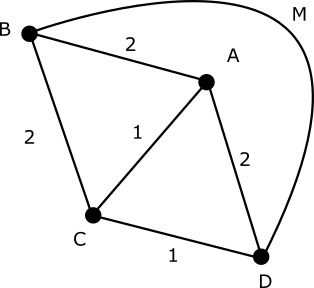
\includegraphics[width=200pt]{ris_example.png}
\end{center}

Рисунок 3.1 - пример графа на котором алгоритм ИБГ не находит оптимальное решение

Рассмотрим данный граф. При начале работы ИБГ из вершины $A$ у нас получится путь $ACDBA$ который зависит от веса $M$ ребра $DB$, которое может быть сколь угодно тяжелым. Оптимальным же маршрутом для данного графа является цикл $ADCBA$

Однако, если мы наложим дополнительные условия на веса ребер или сам граф мы можем получить более точный результат. Исследование асимптотики работы алгоритма ИБГ при некоторых условиях и является целью данной работы. \newline

\newpage

\begin{center}
\addcontentsline{toc}{section}{ОСНОВНАЯ ЧАСТЬ}
\chapter{\textbf{ОСНОВНАЯ ЧАСТЬ}}
\end{center}

\setcounter{section}{0}


\section{Исследование асимптотики алгоритма ИБГ при метрической постановке задачи TSP}

Метрическая постановка задачи коммивояжера отличается от классической тем, что для графа выполняется неравенство треугольника. То есть для любых трех вершин

\begin{equation}
d_{AB} \leq d_{AC} + d_{CB}
\end{equation}

Физические растояния в нашем мире удовлетворяют неравенству треугольника, а значит для многих случаев, в которых задача была поставлена как просто задача коммивояжера можно говорить о метрической постановке задачи. Например, если у нас есть $N$ населенных пунктов и за вес пути между ними принято физическое расстояние между двумя  населенными пунктами и нужно посетить их все, преодолев минимальное расстояние за весь маршрут, данную постановку можно рассматирвать как метрическую, а как следствие, применить нижедоказанные теоремы.

Для метрической постановки задач существуют верхняя и нижняя оценки оптимальности алгоритма ИБГ.[2] \\


\subsection{Верхняя оценка оптимальности}

\textbf{Теорема 1}

Для маршрута коммивояжера с $n$ вершинами справедлива теорема:

\begin{equation}
	(\frac{Greedy}{Optimal}) \leqq \frac{1}{2}\lceil{\lg n}\rceil + \frac{1}{2}
\end{equation}

Где $Greedy$ - вес пути, найденного жадным алгоритмом, $Optimal$ - вес наиболее оптимального пути.

Доказательство:

\textbf{Лемма 1}: Допустим существует отображение вершины $p$ в число $l_p$ такое, что:\\
1) $d(p,q) \geq min(l_p, l_q) \: \forall \: p,q$\\
2) $l_p \leq \frac{1}{2}Optimal\: \forall \: p $\\
Тогда 
\begin{equation}
\sum l_p \leq \frac{1}{2}(\lceil lg(n)\rceil+1)Optimal
\end{equation}

Доказательство.
Допустим б.о.о., что N такое, что  $\{i|1 \leq i \leq n \}$  и $l_i \geq l_j$ если $i \leq j$
Докажем, что 

\begin{equation}\label{metriclowerbound}
	{Optimal} \geqq 2\sum_{i=k+1}^{min(2k,n)}\mathrm{l}_i
\end{equation}

для любого $k$ такого что $l \leq k \leq $n
Пусть H полный подграф, определенный на множестве узлов

\begin{equation}
	{\{i|1 \leq i \leq min(2k, n)\}}
\end{equation}

Пусть $T$ - это маршрут коммивояжера в $H$, который посещает вершины $H$ в том же порядке, что и эти узлы посещаются при оптимальном обходе исходного графа. Обозначим длину маршрута $T$ как LENGTH. По неравенству треугольника каждое ребро (b, c) графа T должно иметь длину меньше или равную длине пути от b до c, вычисленного в оптимальном пути коммивояжера. Так как ребра $T$ суммируются в $LENGTH$, а сумма ребер оптимального пути равна $Optimal$ мы заключаем что
\begin{equation}
	{Optimal} \geqq {LENGTH}
\end{equation}

По условию 1) Леммы для каждого $(i, j)$ в пути T  $d (i, j)\geq min (\mathrm{l}_i, \mathrm{l}_j)$. Следовательно,

\begin{equation}\label{metric2.3}
	{LENGTH} \geqq \sum_{(i,j)\in T}^{}min(\mathrm{l}_i,\mathrm{l}_j ) = \sum_{i\in H}^{} \mathrm{\alpha}_i\mathrm{l}_i
\end{equation}

где $a_i$ - количество ребер $(i, j)$ в $T$, для которых $i > j$ (и, следовательно, $l_i=min(l_i, l_j)$).
Мы хотим получить нижнюю оценку правой части \eqref{metric2.3}. Заметьте, что каждое $a_i$ не превосходит 2 (потому что $i$ это конечная точка только двух ребер в маршруте T) и что сумма $a_i$ равна количеству ребер в $T$. Поскольку $k$ составляет не менее половины количества ребер в $T$, мы заведомо получим нижнюю оценку правой части \eqref{metric2.3}, если мы предположим, что $k$ наибольших $l_i$ имеют $a_i=0$, а остальные $min (2k, n) - k$ из $l_i$ имеют $a_i= 2$. По предположению, $k$ наибольших $\{ l_i|1 \leq i \leq k\}$, поэтому оценка нижней границы:


\begin{equation}
	\sum_{i \in H} a_i l_i \geq 2 \sum_{i=k+1}^{min(2k, n)} l_i
	\label{sum}
\end{equation}

Таким образом мы доказали неравенство \eqref{metriclowerbound}

Теперь просуммируем неравенства \eqref{metriclowerbound} для всех $k$ равных степени двойки меньшей $n$, то есть:
\begin{equation}
\sum_{j=0}^{[lg(n)]-1} Optimal \geq \sum_{j=0}^{[lg(n)]-1} 2* \sum_{i=2^j+1}^{min(2^{j+1}, n)} l_i
\end{equation}

Это можно упростить до

\begin{equation}
\lceil lg(n) \rceil Optimal \geq 2* \sum_{i=2}^{n} l_i
\end{equation}

По условию 2) Леммы
\begin{equation}
Optimal \geq 2*l_1
\end{equation}
Два данных неравенства доказывают лемму

Доказательство Теоремы 1. Для каждой  вершины $p$ положим, что $l_p$ это длина ребра, выходящего из p и идущего в вершину, которая выбирается жадным алгоритмом. Мы хотим показать, что $l_p$ удовлетворяет условиям Леммы 1. Если вершина $p$ была выбрана жадным алгоритмом до вершины $q$, тогда вершина $q$ была кандидатом на ближайшую невыбранную вершину для вершины $p$. Это значит, что ребро $(p,q)$ не короче чем выбранное ребро, то есть
\begin{equation}
d(p,q) \geq l_p
\end{equation}
И наоборот, если вершина $q$ была выбрана до $p$, тогда
\begin{equation}
d(p,q) \geq l_q
\end{equation}
Так как одна из вершин была выбрана раньше другой, одно из двух последних неравенств должно выполняться, вследствие чего  условие 1) Леммы 1 выполняется. Для доказательства условия 2) достаточно доказать, что для любого ребра $(p,q)$
\begin{equation}
d(p,q) \leq \frac{1}{2}Optimal
\end{equation}
Мы можем рассмотреть оптимальный маршрут как объединение двух частей маршрута, каждый из которых это путь между $p$ и $q$. Из неравенства треугольника получаем, что длина любого пути между $p$ и $q$ не может быть меньше, чем $d(p,q)$, что доказывает неравенство выше. Так как $l_p$ это длины всех пар, составляющих маршрут $T$
\begin{equation}
\sum l_p = GREEDY
\end{equation}
Данное равенство вместе с Леммой 1 доказывают неравенство из Теоремы 1.\\

\subsection{Нижняя оценка оптимальности}


\textbf{Теорема 2}

Для маршрута коммивояжера с $n$ вершинами справедлива теорема:

\begin{equation}
	(\frac{Greedy}{Optimal}) > \frac{1}{3}{\lg (n+1)} + \frac{4}{9}
\end{equation}

Доказательство:  Для каждого $i \geq 1 $ построим неполный взвешенный граф F с тремя особыми вершинами: левая вершина, центральная вершина и правая вершина. Эти графы строятся рекурсивно как показано на рисунке 1.1 где левая вершина располагается слева, правая - справа и центральная посередине. Каждый граф F имеет путь P, соединяющий левую вершину и центральную, в который входят все вершины графа. Путь P также строится рекурсивно как на рисунке 1.1 

\begin{center}
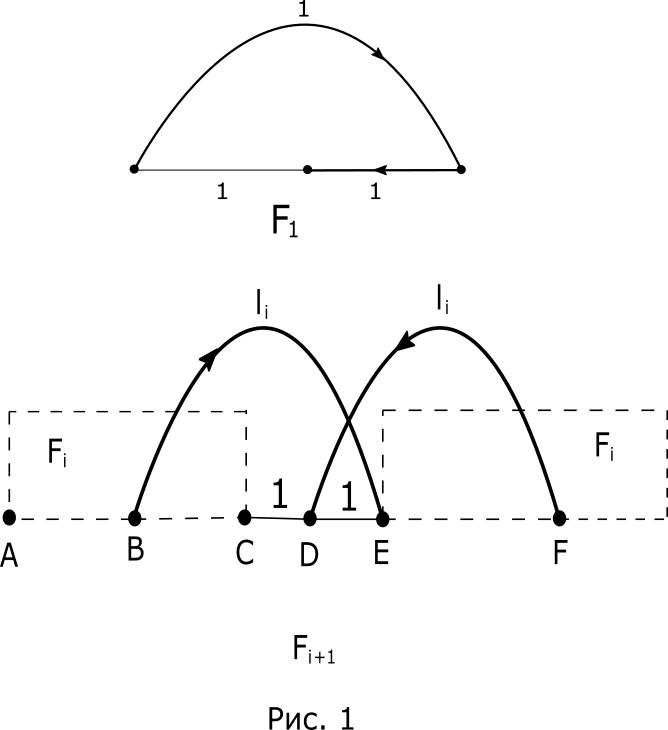
\includegraphics[width=300pt]{ris1.png}
\end{center}

\begin{center}
Рисунок 1.1 - рекурсивное построение графа
\end{center}


Граф $F_1$ состоит из трех вершин, между каждыми двумя из которых проведено ребро веса 1. Путь $P$ состоит из двух ребер: между левой и правой вершиной, между правой и центральной вершиной. Для построения графа $F_{i+1}$ возьмем две копии графа $F_i$, назовем одну копию левой, а другую правой. Добавим дополнительную вершину которая впоследствии станет центральной для $F_{i+1}$. На рисунке 1.1 эта вершина обозначена $D$. Она соединяется с правой вершиной левой копии (вершина $C$) и левой вершиной правой копии (вершина $E$) ребрами длины 1. Дополнительная вершина $D$ также соединяется с центральной вершиной правой копии (вершина $F$) ребром веса $l_i$, который будет определен ниже. Наконец, центральная вершина левой копии (вершина $B$) соединяется с левой вершиной правой копии (вершина $E$) ребром веса $l_i$. Левая вершина $F_{i+1}$ определяется как левая вершина левой копии (вершина $A$), правая вершина $F_{i+1}$ определяется как правая вершина правой копии (вершина $G$). Путь $P_{i+1}$ состоит из двух копий пути $P_i$ и ребер $(B,E)$, $(F,D)$ длины  $l_i$. Длина $l_i$ данных ребер определяется по формуле
\begin{equation}\label{2.11}
l_i = \frac{1}{6}(4*2^i-(-1)^i+3)
\end{equation}
Пусть $L_i$ - длина пути $P_i$. Для длины $L_i$ есть рекуррентное соотношение:
\begin{equation}
L_{i+1} = 2*L_i+2*l_i
\end{equation}
Так как $P_{i+1}$ состоит из двух копий $P_i$ и двух ребер веса $l_i$ При условии что $L_1=2$, решение данного уравнения: 
\begin{equation}
L_i=\frac{1}{9}(6i*2^i+8*2^i+(-1)^i-9)
\end{equation}
Для каждого $F$ мы определяем граф $G_i$, который получается из $F$ путем соединения левой вершины и правой вершины графа ребром веса $1$ и соединением центральной вершины с левой вершиной ребром веса $l_i-1$. Левая вершина графа $F$ считается начальной вершиной графа $G_i$. На рисунке 1.2 изображен граф $G_4$ Определим $\bar G_i$ как полный граф на вершинах $G_i$. Длина ребер в данном графе будет равна длине наименьшего пути в $G_i$ между двумя вершинами, которые соединяет ребро. Таким образом $\bar G_i$ будет удовлетворять неравенству треугольника.


\begin{center}
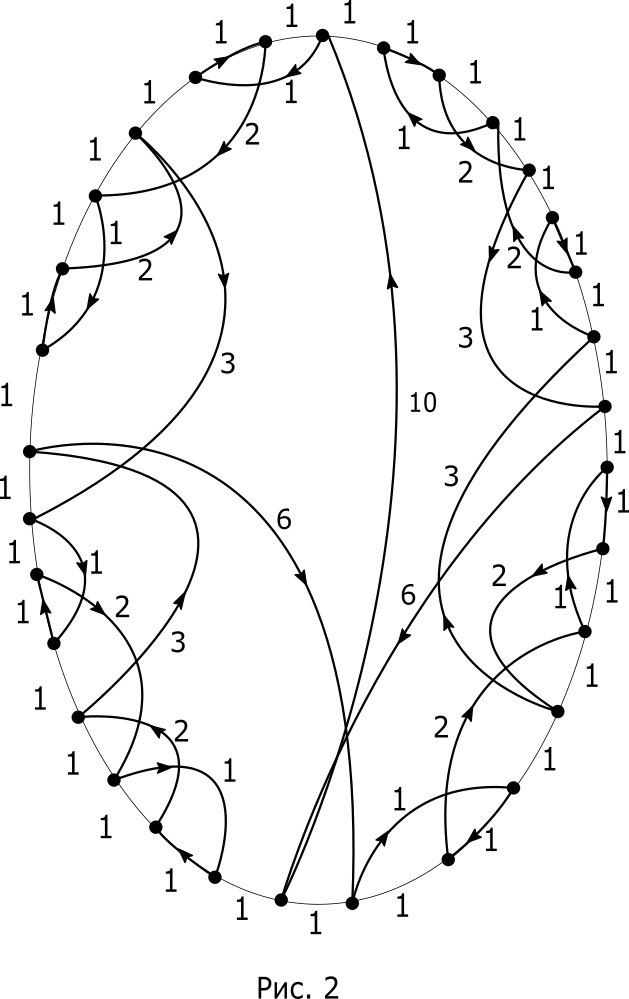
\includegraphics[width=200pt]{ris2.png}
\end{center}

\begin{center}
Рисунок 1.2 - пример графа $G_4$
\end{center}


Граф $\bar G_i$ имеет два важных свойства:\\
1) Ребра графа $G_i$ имеют в графе $\bar G_i$ такие же длины как и в $G_i$ \\
2) Если жадный алгоритм начинает свою работу с начальной вершины графа  $G_i$ то при подходящем выборе меджу несколькими возможными путями в алгоритме метод может найти путь $P_i$, который будет следовать за ребром длины $l_i-1$, проведенным из центральной вершины (последняя в пути $P_i$) в начальную вершину.

Мы вернемся к доказательству этих свойств после завершения доказательства основной теоремы.
Каждый граф $\bar G_i$ имеет оптимальный маршрут, состоящий из ребер единичного веса, с, соответственно весом пути равным $n$, где $n$ - это количество вершин ($2^{i+1}-1$). Данный путь начинается в начальной вершине и далее посещаются все вершины слева направо, после чего происходит возврат в начальную вершину. Примером, удовлетворяющим теореме является граф $\bar G_{m-1}$ Соотношение для него:
\begin{equation}
\frac{GREEDY}{Optimal} = (L_i+l_i-1)/n, \:  i=lg(n+1)-1
\end{equation}
Данное соотношение больше чем соотношение в теореме.
Остается доказать свойства 1) и 2).
Рассмотрим рисунок 1.1
Покажем что для каждого $F_{i+1}$
\begin{equation}\label{2.13}
\overline {AB}= \overline {BC}= \overline {EF}=\overline {FG}=l_i-1
\end{equation}
\begin{equation}\label{2.14}
\overline {AC}= \overline {EG}=l_{i+1}-2
\end{equation}
\begin{equation}\label{2.15}
\overline {BE}= \overline {DF}=l_i
\end{equation}
\begin{equation}\label{2.16}
\overline {AD}= \overline {DG}=l_{i+1}-1
\end{equation}
\begin{equation}\label{2.17}
\overline {AG}=l_{i+2}-2
\end{equation}

\begin{center}
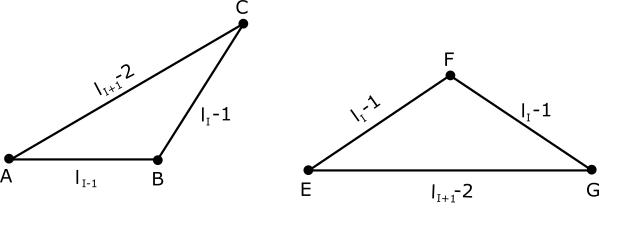
\includegraphics[width=300pt]{ris3.png}
\end{center}

\begin{center}
Рисунок 1.3 - две копии $F_i$ до объединения
\end{center}

\begin{center}
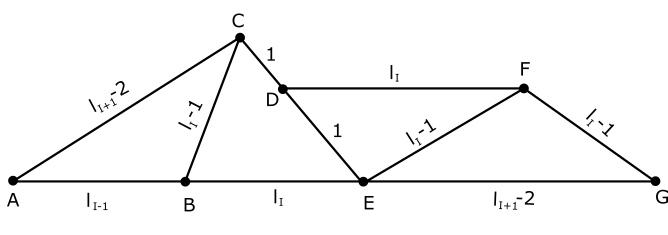
\includegraphics[width=300pt]{ris4.png}
\end{center}

\begin{center}
Рисунок 1.4 - две копии $F_i$ после объединения
\end{center}


Запись $\overline {XY}$ означает длину кратчайшего пути между X и Y в графе $F_{i+1}$. Данные равенства тривиально доказываются для i=1. Далее будем вести доказательство по индукции. Предположим что равенства верны для $i \leq I-1$, например для $F_I$ На рисунке 1.3 изображены связанные вершины графа $F_{I+1}$ до объединения двух копий $F_I$ в $F_{I+1}$. Веса ребер графа равны кратчайшему пути между ними в $F_I$. Эти веса определены в предположении индукции. Например, ребро (A,B) на рисунке 1.3 соединяет левую и центральную вершины $F_I$ и, как следует из \eqref{2.16}, длина кратчайшего пути между этими вершинами равна $l_i-1$. На рисунке 1.4 мы можем увидеть фигуры с рисунка 1.3 с ребрами, которые были добавлены при построении $F_{I+1}$. Так как каждый вес ребра между двумя вершинами на рисунке 1.3 равен кратчайшему пути между этими вершинами, то применяя формулу \eqref{2.11} для $l_I$ ко всем возможным путям в $F_{i+1}$ мы можем найти, что вес каждого ребра на рисунке 1.4  действительно является длиной кратчайшего пути между двумя вершинами, которые соединяет ребро. Это доказывает равенства \ref{2.13}-\ref{2.15} для $F_{I+1}$. Равенства \ref{2.16}, \ref{2.17} доказываются аналогичными рассуждениями для всех путей на рисунке 1.4. Путем длины $l_{i+1}-2$ из $A$ в $G$ является путь $ABEG$.

Также стоит отметить, что  \ref{2.13} - \ref{2.16} выполняются и когда из $F_{I+1}$ строится $G_{I+1}$. Это можно доказать соединив $A$ и $G$ на рисунке 1.4 ребром веса $l_{I+1}-1$ и снова проверив пути. Кратчайшим путем из $A$ в $D$ является ребро $(A,D)$.

Теперь вернемся к свойству а). Уравнение \eqref{2.15} показывает, что для каждого построенного $F_{i+1}$ ребра, добавленные при построении содержатся в кратчайшем пути. Все расстояния между точками в $F_i$ уже вычислены на момент построения $F_{i+1}$ потому, что расстояния между особыми точками уже вычислены. (сравним \eqref{2.13} и \eqref{2.16}, \eqref{2.14} и \eqref{2.17})

Мы уже заметили, что последнее добавленное ребро при построении $G_i$ является кратчайшим путем и, очевидно, путь состоящий из ребер длины $1$ является кратчайшим. Таким образом, свойство 1) доказано.

Свойство 2) доказывается тем фактом, что центральная вершина графа $F_i$ достигается только после посещения всех остальных вершин, и вершина в конце ребра длины $l_i$ хотя бы настолько же близка как любая другая вершина, достигаемая через левую или правую вершины. Эти вершины уже на расстоянии $l_{i-1}$ от центральной вершины и как минимум на расстоянии $1$ от еще не выбранной вершины. \\




\newcommand{\algorithm}{$\mathcal{A}$}
\newcommand{\topboundE}{$\mathcal{Z^*_{A}}$}
\newcommand{\topboundD}{$\mathcal{D^*_{A}}$}
\newcommand{\randomvalue}{$\mathcal{Z_{A}}$}
\newcommand{\randomvalueE}{$E(\text{\randomvalue})$}
\newcommand{\randomvalueD}{$D(\text{\randomvalue})$}

\section{Условия асимптотической оптимальности жадного алгоритма}

Для дальнейшего доказательства некоторых теорем нам потребуются следующие определения и теоремы. Теоремы приведены без доказательства.\\


Алгоритм $\mathcal{A}$ будем называть ассимптотически оптимальным если существуют такие $\epsilon_n \rightarrow 0, \delta_n \rightarrow 0$ при $n \rightarrow \infty$ что применение алгоритма $\mathcal{A}$ дает значение  $\mathcal{Z_A}$, удовлетворяющее неравенству
 
\begin{equation}\label{1}
P\{\mathcal{Z_A} \leq (1+\epsilon_n)\mathcal{Z}\}\geq 1-\delta_n
\end{equation}

где $\mathcal{Z_A}$ - решение, найденное алгоритмом, $\mathcal{Z}$ - минмальное решение.
Это определение при $\epsilon_n \equiv 0$ совпадает с понятием алгоритма, который почти всегда приводит к точному решению. \\

Альтернативный вариант формулы из определения:

\begin{equation}
P\{\mathcal{Z_A} \leq (1+\epsilon_n)\mathcal{Z}\}\leq 1+\delta_n
\end{equation} \\


\textbf{Неравенство Чебышева} \\

Пусть случайная величина X: $\Omega\rightarrow\mathbb {R}$ определена на вероятностном пространстве ( $\Omega,{\mathcal {F}},\mathbb {P} $)
, а её математическое ожидание $\mu$ и дисперсия  $\sigma ^{2}$ конечны. Тогда 
\begin{equation}
{\mathbb {P}}\left(|X-\mu |\geqslant a\right)\leqslant {\frac {\sigma ^{2}}{a^{2}}}
\end{equation},
где  $a>0$. \\ \\


\textbf{Теорема Петрова} \\

Пусть $X_1,...,X_n$ — независимые случайные величины и
существуют положительные постоянные $g_1,...,g_n$ и $T$ такие, что для всех $0 \leq t \leq T$

\begin{equation}
\mathbb {E}e^{tX_k} \leq e^{\frac{1}{2} g_k t^{2}}
\end{equation}

Положим $S=\sum_{k=1}^{n} X_k $ и $G=\sum_{k=1}^{n} g_k $. Тогда

\begin{equation}
P\{S > x\} \leq 
\begin{cases}
   exp (-\frac{x^{2}}{2G}), \; 0 \leq x \leq GT\\
   exp (-\frac{Tx}{2}), \; x\geq GT \\
 \end{cases}
\end{equation}\\


\subsection{Общее условие асимптотической оптимальности}

Найдем условия, при выполнении которых жадный алгоритм является асимптотически оптимальным, то есть
\begin{equation}\label{assymptopt}
P\{\text{\randomvalue} > (1+\epsilon_n)\mathcal{Z}\}\leq \delta_n
\end{equation}
где $\epsilon_n \rightarrow 0, \delta_n \rightarrow 0$ $n \rightarrow \infty$\\

Вес маршрута коммивояжера, полученного применением жадного алгоритма обозначим как $\text{\randomvalue}$. Он определяется формулой
\begin{equation}
\text{\randomvalue} = \sum_{k=1}^n a_{i_k i_{k+1}}
\end{equation}

Вес маршрута отпимального решения задачи обозначим как $\mathcal{Z}$. Он определяется формулой:

\begin{equation}
\mathcal{Z} = \min_{\{ \pi \}} \sum_{k=1}^n a_{i_k i_{k+1}}
\end{equation}


Оценим сверху левую часть \eqref{assymptopt}. Так как $a>0$, то $\mathcal{Z} \geq na$ и 
\begin{equation}\label{4}
P\{\mathcal{Z_{A}} > (1+\epsilon_n)\mathcal{Z}\}\leq P\{\mathcal{Z_{A}} > (1+\epsilon_n)na\}
\end{equation}


Обозначим через\topboundE и \topboundD верхние оценки соответственно математического ожидания \randomvalueE и дисперсии \randomvalueD случайной величины \randomvalue . Обозначим $\Delta_n=(1+\epsilon_n)na-\text{\topboundE}$. Получаем:
\begin{equation}\label{5}
P\{\text{\randomvalue} > (1+\epsilon_n)na\} = 
P\{\text{\randomvalue} > \text{\topboundE}+[(1+\epsilon_n)na-\text{\topboundE}]\} \leq
P\{\text{\randomvalue} > \text{\randomvalueE})+ \Delta_n\}
\end{equation}

Пусть $\epsilon_n = K(\frac{\text{\topboundE}}{na}-1), K>1$.
Тогда $ \Delta_n = (K-1)(\text{\topboundE}-na) \geq 0$.
Продолжим неравенство \eqref{5} применив неравенство Чебышева.
\begin{equation}\label{6}
\begin{aligned}
P\{\text{\randomvalue}> E(\text{\randomvalue})+ \Delta_n\} \leq 
P\{|\text{\randomvalue}- \text{\randomvalueE})| \geq \Delta_n\} \leq \\
\frac{\text{\randomvalueD}}{\Delta^2_n} \leq
\frac{\text{\topboundD}}{\Delta^2_n} = 
\frac{\text{\topboundD}}{(K-1)^2(\text{\topboundE}-na)^2}
\end{aligned}
\end{equation}
Так как $K$ - константа, $K>1$, то из данной цепочки неравенств следует, что условие ассимптотической оптимальности жадного алгоритма будет выполнено если мы покажем, что
$ \epsilon_n=K(\frac{\text{\topboundE}}{na}-1) \rightarrow 0$ и 
$ \delta_n = \frac{\text{\topboundD}}{(K-1)^2(\text{\topboundE}-na)^2} \rightarrow 0$ при $ n \rightarrow \infty$\\

Вычисление верхних оценок \topboundE и \topboundD\\

\newcommand{\chanceLklesserX}{$\Phi_k(x)$}
\newcommand{\randomNormalValueE}{$l_k$}

Математическое ожидание \randomvalueE равно сумме матожиданий величин $a_{{i_k}{i_{k+1}}}$ минимальных длин ребер, ведущих в еще непосещенную вершину на k-м шаге алгоритма \algorithm. В целях удобства дальнейших вычислений пронормируем случайную величину $\xi$ значений элементов $a_{ij}$ длин ребер графа, положив $\xi'=\frac{\xi-a}{b-a}$. Обозначим через \randomNormalValueE  значение матожидания нормированной случайной величины $\text{\randomNormalValueE}=a_{{i_k}{i_{k+1}}}'$. На k-ом шаге алгоритма выбирается минимум из $n-k$ элементов. В силу независимости этих элементов вероятность \chanceLklesserX того, что величина \randomNormalValueE минимального из этих элементов не превышает величины $x$ равна
\begin{equation}
\text{\chanceLklesserX}=P\{\text{\randomNormalValueE} \leq x\}=1-(1-F(x))^{n-k}
\end{equation}
, где
\begin{equation}
F_k(x)=P\{\xi' \leq x\}, 0\leq x 
\leq 1
\end{equation}
Тогда величина $E(\text{\randomNormalValueE})$ равна
\begin{equation}
E(\text{\randomNormalValueE})=\begin{cases}
\int_0^1 x d\text{\chanceLklesserX}, k=1,2,...n-1 \\
E(l_{n-1}), при k=n
\end{cases}
\end{equation}
откуда получим
\begin{equation}\label{7}
\begin{aligned}
E(\text{\randomNormalValueE}) = x \text{\chanceLklesserX}\rvert_{0}^{1}-\int_0^1 \text{\chanceLklesserX}dx = \\
=1-\int_0^1 [1-(1-F(x))^{n-k}]dx = \int_0^1 (1-F(x))^{n-k}]dx \\
k = \overline {1, n-1}
\end{aligned}
\end{equation}
В силу нормировки минимальный элемент $a_{i_{k-1} i_k}$ связан с величиной  \randomNormalValueE  соотношением $a_{i_k i_{k+1}} = a+(b-a)\text{\randomNormalValueE}$. Поэтому
\begin{equation}\label{8}
\text{\randomvalueE} = \sum_{k=1}^{n} [a+(b-a)E(\text{\randomNormalValueE})]
\end{equation}.
Откуда с учетом \eqref{7} имеем:
\begin{equation}
\begin{aligned}
\text{\randomvalueE} = na+(b-a)[\int_0^1 \sum_{k=1}^{n-1}(1-F(x))^{n-k}dx + \int_0^1 (1-F(x))dx]=\\
=na+(b-a) \int_0^1 \frac{[1-F(x)][1-(1-F(x))^{n-1}+F(x)]}{F(x)}dx \leq \\
\leq na + (b-a) \int_0^1 \frac{1-(1-F(x))^n}{F(x)}dx = \\
=na+(b-a)[\int_0^{\gamma_n} \frac{1-(1-F(x))^n}{F(x)}dx + 
\int_{\gamma_n}^1 \frac{1-(1-F(x))^n}{F(x)} dx]
\end{aligned}
\end{equation}
где $\gamma_n$ - корень уравнения $F(\gamma) = \frac{1}{n}$, то есть $\gamma_n = F^{-1}(\frac{1}{n})$. Учитывая что при $0 \leq Z \leq 1$ справедливо неравенство $\frac{1-(1-Z)^n}{Z} \leq n$, оценку $E( {\mathcal{Z_{A}}})$ можем продолжить следующим образом
\begin{equation}\label{9}
\text{\randomvalueE} \leq \text{\topboundE} = na+(b-a)[\gamma_n * n+ \int_{\gamma_n}^1 \frac{dx}{F(x)}]
\end{equation}

Перейдем к вычислению верхней оценки $\mathcal{D_A^{*}}$. Дисперсия $d_k$ случайной нормированной величины $l_k$ на k-ом шаге равна
\begin{equation}
d_k=\int_0^1 (x-E(l_k))^2 d \Phi_k(x) = \int_0^1 x^2 d \Phi_k(x)- (E(l_k))^2 < \int_0^1 x d \Phi_k(x) = E(l_k)
\end{equation}

Тогда с учетом того, что дисперсия минимального элемента $a_{i_k i_{k+1}}$ равна $(b-a)^2 d_k$, дисперсия случайной величины ${\mathcal{Z_{A}}}$ с учетом \eqref{8} оценивается следующим образом:
\begin{equation}
\begin{aligned}
\mathcal{D(\mathcal{Z_{A}})} = \sum_{k=1}^n (b-a)^2 d_k < (b-a)^2 \sum_{k=1}^n E(l_k) =\\
= (b-a)^2 * \frac{E(\mathcal{Z_{A}})-na}{(b-a)} \leq (b-a)(\mathcal{Z_{A}^*}-na)
\end{aligned}
\end{equation}

Окончательно с учетом \eqref{9} получаем верхнюю оценку для $\mathcal{D(\mathcal{Z_{A}})}$
\begin{equation}\label{10}
\mathcal{D(\mathcal{Z_{A}})} < \mathcal{D_{A}^*} = (b-a)^2 [\gamma_n*n+\int_{\gamma_n}^1 \frac{dx}{F(x)}]
\end{equation}
Вернемся к неравенству \eqref{6}. Имея в виду полученные оценки \eqref{9} и \eqref{10}, выражения для $\epsilon_n$ и $\delta_n$ можно записать в следующем виде: 
\begin{equation}
\epsilon_n = K(\frac{b}{a}-1)[\gamma_n + \frac{1}{n} \int_{\gamma_n}^1 \frac{dx}{F(x)}]
\end{equation}
\begin{equation}
\delta_n = \frac{1}{(K-1)^2 [\gamma_n * n + \int_{\gamma_n}^1 \frac{dx}{F(x)}]}
\end{equation}

Обозначим $\mathcal{I}_n = \int_{\gamma_n}^1 \frac{dx}{F(x)}$, $\Psi(n)$ - произвольная растущая от n функция, $\lim\limits_{x\to \infty} \Psi(n) = \infty $ \\

\textbf{Теорема 1}

Алгоритм $\mathcal{A}$ является асимптотически оптимальным при выполнении условий $\lim\limits_{{n} \to \infty} \mathcal{I}_n = \infty $ и 
\begin{equation}
\frac{b}{a} \leq \frac{1}{\Psi(n)} min \{ \frac{1}{\gamma_n}, \frac{n}{\mathcal{I}_n} \}
\end{equation}

Доказательство. Покажем, что при выполнении условий теоремы $\epsilon_n \to 0$ и $\delta_n \to 0$ с ростом n. Действительно, при $K>1$ имеем:

\begin{equation}
\begin{aligned}
\delta_n = \frac{1}{(\gamma_n n+\mathcal{I}_n)(K-1)^2} \leq \frac{1}{\mathcal{I}_n * (K-1)^2} \to 0 \\
\epsilon_n = K(\frac{b}{a}-1)(\gamma_n+\frac{1}{n} \mathcal{I}_n) \leq K*\frac{b}{a} (\gamma_n+\frac{1}{n} \mathcal{I}_n)\leq \\
\leq \frac{K}{\Psi(n)} min(\frac{1}{\gamma_n}, \frac{n}{\mathcal{I}_n})(\gamma_n+\frac{1}{n} \mathcal{I}_n) = \\
= \frac{K}{\Psi(n)} min (1+\frac{\mathcal{I}_n}{n \gamma_n}, 1+\frac{n \gamma_n}{\mathcal{I}_n}) \leq \frac{2K}{\Psi(n)} \to 0
\end{aligned}
\end{equation}
при $n \to \infty$. Теорема 1 доказана.

Замечание. Как было показано выше, для своей работы алгоритм $\mathcal{A}$ требует $O(n^2)$ операций, что сравнимо с трудоемкостью записи исходной информации о задаче коммивояжера. Отсюда получаем, что при выполнении условий теоремы 1 алгоритм $\mathcal{A}$ является статистически эффективным.\\


\subsection{Вероятностный анализ ИБГ для равномерного распределения}


Определим условия асимптотической оптимальности алгоритма $\mathcal{A}$ для случая, когда веса ребер графа $a_{ij}$ могут быть выбраны равновероятно из отрезка [a,b], a>0. В этом случае нормированная интегральная функция распределения имеет вид $F(x) = x,\; 0 \leq x \leq 1,\; \gamma_n = F(\frac{1}{n}) = \frac{1}{n}$ и
\begin{equation}
\mathcal{I}_n = \int_{\gamma_n}^1 \frac{dx}{F(x)} = \int_{\frac{1}{n}}^1 \frac{dx}{x} = ln(n)
\end{equation}

Тогда из теоремы 1 непосредственно получаем результат, который может быть сформулирован как:\\

\textbf{Теорема 2}

Если элементы $a_{ij}$ матрицы А принимают значения равновероятно из отрезка [a,b], то алгоритм $\mathcal{A}$ является асимптотически оптимальным при выполнении следующего условия:
\begin{equation}
\frac{b}{a} \leq \frac{n}{ln(n)}•\frac{1}{\Psi(n)}
\end{equation}

Представляет интерес оценить величины $\epsilon_n$ и $\delta_n$, фигурирующие в соотношении \eqref{1}.

Учитывая специфику равномерного распределения можно получить более точные оценки для этих величин по сравнению с общим случаем. Выведем условия асимптотической оптимальности алгоритма $\mathcal{A}$ в случае равномерного распределения, проведя в сокращенном виде вычисления оценок для $E(\mathcal{Z_{A}})$ и $\mathcal{D(Z_{A})}$ и $P \{ \mathcal{Z_{A}} \leq (1+\epsilon_n)\mathcal{Z} \}$. Согласно \eqref{7}
\begin{equation}\label{eq13} 
E(l_k) = \int_0^1 (1-x)^{n-k}dx = \int_0^1 x^{n-k}dx = \frac{1}{n-k+1}
\end{equation}
$k=1,2,...n-k$;   $ E(l_n) = E(l_n-1) = \frac{1}{2}$

С учетом \eqref{8}
\begin{equation}
\begin{aligned}
E(\mathcal{Z_{A}}) = \sum_{k=1}^{n} [a+(b-a)E(l_k)] = na +(b-a)(\frac{1}{2}+\sum_{k=1}^{n-1} \frac{1}{n-k+1}) \leq \\
\leq na+(b-a)(\frac{1}{2} + ln(n)) = \mathcal{Z^*_{A}}
\end{aligned}
\end{equation}

Оценим дисперсию $d_k=\int_0^1 (x-E(l_k))^2 d\text{\chanceLklesserX}$ случайной величины $l_k$ с учетом того, что для равномерного распределения \chanceLklesserX $ = 1-(1-x)^{n-k}$

Используя \eqref{eq13}, имеем
\begin{equation}
\begin{aligned}
d_k = \int_0^1 x^2 d \text{\chanceLklesserX}-E(l_k)^2=x^2 \text{\chanceLklesserX} 	
|_0^1 - 2 \int_0^1 x \text{\chanceLklesserX}dx - E(l_k)^2=\\
= 1-2\int_0^1 x[1-(1-x)^{n-k}]dx-E(l_k)^2 =\\
= \frac{2}{n-k+1} - \frac{2}{n-k+2} - \frac{1}{(n-k+1)^2}, \\ 
\; k=1,2,...,n-1; \; d_n = d_{n-1} = \frac{1}{12}
\end{aligned}
\end{equation}

Отсюда с учетом определения дисперсии величины \randomvalue , получим
\begin{equation}
\begin{aligned}
\frac{1}{(b-a)^2} \text{\randomvalueD} = \sum_{k=1}^n d_k = \frac{1}{12} + \sum_{k=1}^{n-1} (\frac{2}{n-k+1} - \frac{2}{n-k+2} - \frac{1}{(n-k+1)^2}) = \\
= \frac{1}{12} - \frac{2}{n+1} +1 - \sum_{k=1}^{n-1} \frac{1}{(n-k+1)^2} \leq \frac{13}{12} - \frac{2}{n+1} - \frac{1}{4} - \int_3^{n+1} \frac{dx}{x^2} = \\
= \frac{13}{12} - \frac{2}{n+1} - \frac{1}{4} + \frac{1}{n+1} - \frac{1}{3} < 0.417 = \frac{\text{\topboundD}}{(b-a)^2} 
\end{aligned}
\end{equation}

Приведем оценку вероятности невыполнения соотношения \eqref{1} для случая равномерного распределения:
\begin{equation}\label{14}
\begin{aligned}
P\{ \text{\randomvalue} > (1+\epsilon_n) \mathcal{Z} \} \leq P\{ \text{\randomvalue} > (1+\epsilon_n)na \} \leq \\
\leq P\{ \text{\randomvalue} + \text{\topboundE} - \text{\randomvalueE} > (1+\epsilon_n)na \} = \\
= P \{ \text{\randomvalue} - \text{\randomvalueE} > (1+\epsilon_n)na - \text{\topboundE} \} \leq \\
\leq P \{ |\text{\randomvalue} - \text{\randomvalueE}| > (1+\epsilon_n)na - \text{\topboundE} \} \leq \\
\leq \frac{\text{\randomvalueD}}{[(1+\epsilon_n)na + \text{\topboundE}]^2} \leq \\
\leq \frac{0.417(b-a)^2}{[1+\epsilon_n)na-(nu+(b-a)(\frac{1}{2}+ln(n)))]^2} = \\
= \frac{0.417}{[\frac{n\epsilon_n}{\frac{b}{a}-1}-ln(n) -\frac{1}{2}]^2}
\end{aligned}
\end{equation}

Положим $\epsilon_n = \frac{c}{\Psi(n)}$, константа c>1, и пусть $\frac{a}{b} \leq \frac{n}{ln(n)} • \frac{1}{\Psi(n)}$. Тогда \eqref{14} может быть продолжено следующим образом:

\begin{equation}
\frac{0.417}{[\frac{n\frac{c}{\Psi(n)}}{(\frac{b}{a}-1)}-\frac{1}{2}-ln(n)]} \leq \frac{0.417}{[\frac{c•\frac{b}{a}•ln(n)}{(\frac{b}{a}-1)}-\frac{1}{2}-ln(n)]^2} = \frac{0.417}{[(c-1)ln(n)-\frac{1}{2}]^2} = \delta_n
\end{equation}

Таким образом, окончательная оценка для вероятности выполнения соотношения \eqref{1} примет вид:
\begin{equation}\label{15}
P \{ \text{\randomvalue} \leq (1+\epsilon_n)\mathcal{Z} \} \geq 1 - \frac{0.417}{[(c-1)ln(n)-\frac{1}{2}]^2}
\end{equation}

Нетрудно заметить, что эта величина, характеризующая точность получаемого решения, улучшается с ростом $\Psi(n)$, но при этом ухудшается оценка для величины $\frac{b}{a}$. Выберем функцию $\Psi(n)$ таким образом, чтобы произведение верхних оценок для $\epsilon_n$ и $\frac{b}{a}$ стремилось к \eqref{1} с ростом n. Такому условию отвечает функция $\Psi(n) = \sqrt{\frac{cn}{ln(n)}}$. При этом оценки для $\epsilon_n$ и $\frac{b}{a}$ принимают вид:
\begin{equation}\label{16}
\frac{b}{a} \leq \sqrt{\frac{n}{cln(n)}}
\end{equation}
\begin{equation}\label{17}
\epsilon_n \leq \sqrt{\frac{cln(n)}{n}}
\end{equation}

Анализ соотношений \ref{15}-\ref{17}, полученных для равномерного распределения показывает, что уменьшение константы $c$ "улучшает" оценки для $\frac{b}{a}$ и $\epsilon_n$ и "ухудшает" оценку вероятности $P \{ \text{\randomvalue} \leq (1+\epsilon_n)\mathcal{Z} \}$\\


\subsection{Вероятностный анализ ИБГ для $\beta$ - распределения}


 Очень часто в опытно-конструкторских разработках в промышленности и научно-исследовательских проектах длительности $a_{ij}$ отдельных операций предполагается распределенными по закону: $\beta$ - распределение :
\begin{equation}
f(\xi) = 
\begin{cases}
   \frac{(\xi-a)^\alpha*(b-\xi)^\gamma}{(b-a)^{\alpha+\gamma+1} \beta(\alpha+1, \gamma+1)},  \; \xi \in [a,b]\\
   0, \; \xi \notin [a,b] \\
 \end{cases}
\end{equation}

где
\begin{equation}
\beta(\alpha, \gamma) = \int_0^1 x^{\alpha-1} (1-x)^{\gamma-1} dx = \frac{\Gamma(\alpha)\Gamma(\gamma)}{F(\alpha+\gamma)}
\end{equation}

где $\alpha$ и $\gamma$ - параметры распределения. В нормированном виде функция плотности $f(\xi)$ запишется следующим образом:

\begin{equation}
f(\xi') = 
\begin{cases}
   \frac{(\xi)^\alpha (1-\xi)^\gamma}{ \beta(\alpha+1, \gamma+1)}, \;  \xi' \in [0,1]\\
   0, \;  \xi' \notin [0,1] \\
 \end{cases}
\end{equation}

Рассмотрим частный случай $\beta$ - распределения, когда $\gamma=0$, $\alpha>0$. В этом случае интегральная функция распределения равна
\begin{equation}
F(x) = \int_0^x f(\xi')d\xi' = \int_0^x \frac{x}{\beta(\alpha+1,1)} = x^{\alpha+1}
\end{equation} 
Вычислим величину $\gamma_n$, фигурирующую в условиях теоремы 1:
\begin{equation}
\gamma_n = F^{-1}(\frac{1}{n}) = \frac{1}{\sqrt[\alpha+1]{n}}
\end{equation}
Тогда первое из условий теоремы 1 выполняется в силу $\alpha>0$
\begin{equation}
\mathcal{I}_n = \int_{\gamma_n}^1 \frac{dx}{F(x)} = \int_{\gamma_n}^1 \frac{dx}{x^{\alpha+1}} = \frac{1}{\alpha} (n^{\frac{\alpha}{\alpha+1}}-1) \rightarrow \infty, \; \; n\rightarrow \infty
\end{equation}

Второе условие принимает вид:

\begin{equation}
\begin{aligned}
\frac{b}{a} \leq \frac{1}{\Psi(n)}•min(\sqrt[\alpha+1]{n}, \frac{\alpha n}{n^{\frac{\alpha}{\alpha+1}}-1}) = \\
=\frac{\sqrt[\alpha+1]{n}}{\Psi(n)} min(1, \frac{\alpha}{1-n^{-\frac{\alpha}{\alpha+1}}})
\end{aligned}
\end{equation}

Учитывая, что

\begin{equation}
min(1, \frac{\alpha}{1-n^{-\frac{\alpha}{\alpha+1}}}) \geq min(1, \alpha)
\end{equation}

Получаем следующее условие асимптотической оптимальности алгоритма \text{\algorithm} для $\beta$ - распределения в частном случае $\gamma=0$, $\alpha>0$:
\begin{equation}
\frac{b}{a} \leq \frac{\sqrt[\alpha+1]{n}}{\Psi(n)}min(1,\alpha)
\end{equation}


\subsection{Вероятностный анализ ИБГ для показательного распределения}


\textbf{Теорема 3}: Задача Random Min TSP в случае показательного распределения весов ребер на $[a_n,\infty)$ решается алгоритмом ИБГ за $O(n^2)$ с оценками относительной погрешности
\begin{equation}
\epsilon_n = 5 \frac{\alpha_n/a_n}{n/ln(n)}
\end{equation}

и вероятности несрабатывания
\begin{equation}
\delta_n = O(n^{-1})
\end{equation}

асимптотически точно при условии
\begin{equation}
\frac{\alpha_n}{a_n} = o(\frac{n}{ln(n)})
\end{equation}

Доказательство:

Пусть $w_{ij}$ - вес ребра $(i, j)$ исходного графа с плотностью распределения
\begin{equation}
p(x) = \begin{cases}
\frac{1}{\alpha_n} e^{-\frac{x-a_n}{\alpha_n}}, \; a_n \leq x \leq \infty \\
0, \; x < a_n
\end{cases}
\end{equation}

Пусть $c_{ij}$ - нормированная величина $w_{ij}$. $c_{ij} = \frac{w_{ij}-a_n}{\alpha_n}$  с плотностью распределения

\begin{equation}
p(x) = \begin{cases}
 e^{-x}, \; 0 \leq x \leq \infty \\
0, \; x < 0
\end{cases}
\end{equation}

И функцией распределения:

\begin{equation}
F(x) = \begin{cases}
 1-e^{-x}, \; 0 \leq x \leq \infty \\
0, \; x < 0
\end{cases}
\end{equation}

Пусть $w_{\pi_k, \pi_{k+1}}$ - вес ребра, выбранного ИБГ на k-ом шаге.

$c_{\pi_k, \pi_{k+1}}$ - нормированный вес ребра, выбранного ИБГ на k-ом шаге.

Вес гамильтонова цикла, построенного ИБГ равен:

\begin{equation}
\begin{aligned}
W(\pi) = \sum_{k=1}^{n-1} w_{\pi_k, \pi_{k+1}} + w_{\pi_n, \pi_{1}} = \\
= \sum_{k=1}^{n-1} (\alpha_n c_{\pi_k, \pi_{k+1}} + a_n) +\alpha_n c_{\pi_n, \pi_{1}} + a_n = \\
= na_n + \alpha_n( \sum_{k=1}^{n-1} c_{\pi_k, \pi_{k+1}} + c_{\pi_n, \pi_1}) = \\
= na_n + \alpha_n S
\end{aligned}
\end{equation}

где

\begin{equation}
S = \sum_{k=1}^{n-1} c_{\pi_k, \pi_{k+1}} + c_{\pi_n, \pi_1}
\end{equation}

Оценим оптимльное решение.

\begin{equation}
OPT \geq na_n
\end{equation}

Оценим вероятность несрабатывания алгоритма
\begin{equation}
\begin{aligned}
P\{ W(\pi)>(1+\epsilon_n)OPT \} \leq \\
\leq P\{na_n + \alpha_n S > (1+\epsilon_n)OPT \} \leq \\ 
\leq P\{na_n + \alpha_n S > (1+\epsilon_n)na_n \} \leq \\
\leq P\{\alpha_n S > na_n\epsilon_n \} \leq \\
\leq P\{S >\frac{na_n\epsilon_n}{\alpha_n}  \} = \\
= P\{\tilde{S} >\frac{na_n\epsilon_n}{\alpha_n} - ES  \}
\end{aligned}
\end{equation}

Оценим $ES$
\begin{equation}
\begin{aligned}
ES = E( \sum_{k=1}^{n-1} c_{\pi_k, \pi_{k+1}} + c_{\pi_n, \pi_1} ) =\\
=  \sum_{k=1}^{n-1} E(c_{\pi_k, \pi_{k+1}}) + E(c_{\pi_n, \pi_1}) = \\
= \sum_{k=1}^{n-1} E(X_1(k)) + E(c_{\pi_n, \pi_1})
\end{aligned}
\end{equation}

где $X_1(k)$ - минимум из $k$ случайных независимых переменных.
\begin{equation}
F_{X_1(k)} = 1 - (1-F(x))^k = 1 - e^{-kx}, \; x \geq 0
\end{equation}

\begin{equation}
EX_1(k) = \int_0^\infty xd(F_{X_1(k)}) =\int_0^\infty xd(1-e^{-kx}) = \frac{1}{k}
\end{equation}

Величина $c_{\pi_n, \pi_1}$ распределена по показательному закону. Найдем матожидание:

\begin{equation}
Ec_{\pi_n, \pi_1} = Ep(x) = \int_0^\infty xe^{-x}dx = 1
\end{equation}

\begin{equation}
\begin{aligned}
\sum_{k=1}^{n-1} E(X_1(k)) + E(c_{\pi_n, \pi_1}) \leq \\
 \leq \sum_{k=1}^{n-1} \frac{1}{k} + 1 \leq \\
 \leq ln(n) + C + 1
\end{aligned}
\end{equation}
Где $C < 0.58$
\begin{equation}
ES \leq ln(n) + C + 1
\end{equation}

\begin{equation}
\begin{aligned}
P\{\tilde{S} >\frac{na_n\epsilon_n}{\alpha_n} - ES  \} \leq \\
P\{\tilde{S} >\frac{na_n\epsilon_n}{\alpha_n} - ln(n) - C - 1  \} \end{aligned}
\end{equation}

Подставим $\epsilon_n$ из условия.
\begin{equation}
\epsilon_n = 5 \frac{\alpha_n/a_n}{n/ln(n)}
\end{equation}
По определению вероятности несрабатывания $\epsilon_n \rightarrow 0$ при $n \rightarrow \infty$

Данное условие выполняется, так как по условию теоремы $\frac{\alpha_n}{a_n} = o(\frac{n}{ln(n)})$.

\begin{equation}
\begin{aligned}
P\{\tilde{S} >5ln(n) - ln(n) - C - 1  \} = \\
P\{\tilde{S} >4ln(n) - C - 1  \}
\end{aligned}
\end{equation}

Применим теорему Петрова при $x = 4ln(n) - C - 1 $.

Нас интересует асимптотика, а значит большие значения $H$, поэтому мы можем рассмотреть только случай $x \geq HT$.
\begin{equation}
P\{\tilde{S} >x \} \leq e^{-\frac{Tx}{2}}
\end{equation}

\textbf{Лемма}[3]. Пусть $T = \frac{1}{2\alpha_n}$ и $g_k = \frac{3\alpha_n^2}{k^2}$, $1 \leq k \leq n-2$. Тогда при любых $k$ и $t$ где $k=1,..,n-2$ и $0 \leq t \leq T$, справедливо неравенство:
\begin{equation}
Ee^{t[\xi_k-E\xi_k]} \leq exp(\frac{g_k t^2}{2})
\end{equation}


Доказательство данной леммы означает, что для $T = \frac{1}{2\alpha_n}$, $X_i = \xi_k-E\xi_k$ и $h_i = \frac{3\alpha_n^2}{k^2}$ выполняется условие теоремы Петрова.

Подставим найденные значения в оценку асимптотики.

В нормированном случае $T = \frac{1}{2}$.

\begin{equation}
P\{\tilde{S} >x \} \leq e^{-\frac{x}{4}}
\end{equation}

Подставим $x$.

\begin{equation}
P\{\tilde{S} >4ln(n) - C - 1 \} \leq e^{-\frac{4ln(n) - C - 1}{4}} \leq e^{-ln(n)} \leq n^{-1} = O(n^{-1})
\end{equation}

Таким образом, мы доказали, что
\begin{equation}
P\{ W(\pi)>(1+\epsilon_n)OPT \} = O(n^{-1})
\end{equation}\\



\section{Вычислительный эксперимент}


Для точного решения задачи TSP в период с 1999 по 2003 года профессором Университета Райса Уильямом Куком была разработана программа под названием "Concorde". Алгоритм решения базируется на "Cutting-Plane" методе математической оптимизации. Результат работы данной программы брался за оптимальный при дальнейших исследованиях.

Для опытов была разработана надстройка над "Concorde"  которая может генерировать необходимый входной файл, вызывать "Concorde"  решать по файлу задачу методом ИБГ и сравнивать полученные результаты.

В случае исследования показательного распределения возникли затруднения с применением "Concorde". Приложение не может обрабатывать слишком большие веса ребер, вследствие чего возникла необходимость использования другого механизма решения. Был найден github репозиторий с реализованным на языке программирования python алгоритмом Хелда-Карпа. Данный алгоритм находит точное решение задачи за время $O(n^2 2^n)$. Опыты подтвердили оценку скорости работы в $O(n^2 2^n)$. В самой работе приводится лишь статистический итог. Алгоритм был запущен для 100 случайных сгенерированных постановок, удовлетворяющих условию. Для размерностей свыше 20 использовался доработанный алгоритм генерации графа и "Concorde" по причине слишком большого времени работы алгоритма, написанного на "Python". Появилась некоторая погрешность при генерации графа, но она становится малозначимой на большой размерности. Результаты работы алгоритмов и некоторая статистика приведены в таблице 3.1.\\

\noindent Таблица 3.1 - Опытные данные, полученные при решении 100 случайных постановок
\begin{center}
 \begin{tabular}{||c c c c||} 
 \hline
 Тип распределения & Размерность графа  & 1+$\epsilon$  & Превышений 1+$\epsilon$ \\ [0.5ex] 
 \hline\hline
 равномерное & 5 & 2.28755032994 & 0 \\ 
 \hline
 равномерное & 10 & 1.9210340371976 & 0 \\
 \hline
 равномерное & 20 & 1.599146454710 & 0 \\
 \hline
 равномерное & 40 & 1.36888794541 & 0 \\
 \hline
 равномерное & 80 & 1.2191013317 & 0 \\
 \hline
 равномерное & 160 & 1.12687934538 & 0 \\
 \hline
 равномерное & 320 & 1.07210401244 & 0 \\
 \hline
 показательное & 5 & 2.6094379124341 & 2 \\
 \hline
 показательное & 10 & 2.151292546497 & 11 \\
 \hline
 показательное & 20 & 1.7489330683884 & 5 \\ 
  \hline
 показательное & 40 & 1.4611099317 & 2 \\ 
  \hline
 показательное & 80 & 1.27387666466 & 0 \\ 
  \hline
 показательное & 160 & 1.1585991817 & 0 \\ 
 \hline
 показательное & 320 & 1.09013001555 & 0 \\[1ex] 
 \hline
\end{tabular}\\
\end{center}



В случае показательного распределения можно наблюдать уменьшение количества несрабатываний вместе с ростом размерности графа. Это соотносится с выводами, полученными в ходе аналитического исследования задачи. 

Отсутствие несрабатываний в случае равномерного арспределения можно объяснить тем, что оценка имеет место быть при $n \rightarrow \infty$. На малых размерностях оценка может быть более грубой нежели на больших. Рассмотрим например графы размерности $5$. Эксперимент проводился для случайных весов, взятых в промежутке $[1;2]$. Верхняя оценка веса маршрута коммивояжера, найденного ИБГ равна $10$. Такая оценка достигается если каждое ребро в маршруте будет максимально по весу, то есть вес равен $2$, ребер в маршруте $5$. Нижняя оценка оптимального решения равна $5$. Если все ребра в оптимальном маршруте веса $1$. Таким образом верхняя оценка на отношение $\frac{Greedy}{Optimal}$ равна $\frac{10}{5} = 2$. Тогда как $\epsilon = \frac{\frac{b}{a}}{\frac{n}{ln(n)}} = 2.28755032994728$. При таких начальных условиях превышения $\epsilon$ не произойдет ни при каком наборе весов ребер из отрезка $[1;2]$. Данное наблюдение также соотносится с выводами из аналитических исследований.

Таким образом, полученные опытные данные кореллируют с данными, которые были получены в аналитической части работы.

\newpage

\begin{center}
\addcontentsline{toc}{section}{ЗАКЛЮЧЕНИЕ}
\chapter{\textbf{ЗАКЛЮЧЕНИЕ}}
\end{center}

Задача коммивояжера - одна из самых известных комбинаторных задач. 
Она имеет много применений в реальной жизни. По этой причине решение данной задачи имеет большое прикладное значение. Задача TSP принадлежит к классу NP-трудных, а значит найти точное решение задачи - это трудозатратная операция. Однако в некоторых случаях вполне достаточно найти приближенное решение, если при этом произойдет существенное ускорение процесса. В данной работе было доказано, что в том случае если в нашем графе большое количество ребер и веса их распределены по равномерному распределению, $\beta$ - распределению или показательному распределению оправдано применение алгоритма ИБГ. Были получены условия асимптотической оптимальности для данных распределений.

В ходе опытных исследований были проведены сравнения результатов работы алгоритма ИБГ и оптимального решения. Результаты опытов подтверждают аналитические данные, полученные ранее.

Интерес для дальнейших исследований представляет поиск условий асимптотической оптимальности для других распределений. Также определенный интерес вызывает более точная оценка $\epsilon$ для случаев $\beta$ - распределения и показательного распределения.



\newpage

\begin{center}
\addcontentsline{toc}{section}{СПИСОК ИСПОЛЬЗОВАННЫХ ИСТОЧНИКОВ И ЛИТЕРАТУРЫ}
\chapter{\textbf{СПИСОК ИСПОЛЬЗОВАННЫХ ИСТОЧНИКОВ И ЛИТЕРАТУРЫ}}
\end{center}

\textbf{Статьи из журнала:}

1 Э. Х. Гимади, А. Ле Галлу, А. В. Шахшнейдер, “Вероятностный анализ одного алгоритма приближённого решения задачи коммивояжёра на неограниченных сверху входных данных”, Дискретн. анализ и исслед. опер., 15:1 (2008), 23–43; J. Appl. Industr. Math., 3:2 (2009), 207–221

2 Rosenkrantz, Daniel J.; Stearns, Richard E.; Lewis, II, Philip M -- An Analysis of Several Heuristics for the Traveling Salesman Problem. September 1977 SIAM Journal on Computing 6(3):563-581

3 Э. Х. Гимади, В. А. Перепелица, “Асимптотический подход к решению задачи коммивояжера”, Управляемые системы, 1974, № 12, 35–45

4 Gutin Gregory, Bang Jie, Yeo Anders. When the greedy algorithm fails., Discrete Optimization, 2004, Volume 1, Issue 2. 121-127

5 Gutin Gregory, Yeo Anders, Zverovich Alexey. Traveling Salesman Should not be Greedy: Domination Analysis of Greedy-Type Heuristics for the TSP. Discrete Applied Mathematics. 117., 2002. 81-86.\\


\textbf{Книги:}

1 Johnson David, Gutin Gregory, McGeoch L.A., Yeo A., Zhang Weixiong, Zverovitch, A.. The travelling salesman problem and its variations. Kluwer Academic Publishers, 2002. 830с.

2 William J. Cook. In Pursuit of the Traveling Salesman: Mathematics at the Limits of Computation. Princeton, 2012. 228с.

3 Гимади Э. Х., Хачай М. Ю. Экстремальные задачи на множествах перестановок. Екатеринбург: “Издательство УМЦ УПИ”, 2016. 220 с.\\

\textbf{Ссылки на электронные ресурсы:}

1 Carl Ekerot Реализация алгоритма Хельда-Карпа на языке программирования "Python". 2016. URL:https://github.com/CarlEkerot/held-karp (дата обращения: 23:05:2021)

2 Gerhard Reinelt Руководство по использованию программы "Concorde". 1995.URL:http://comopt.ifi.uni-heidelberg.de/software/TSPLIB95/tsp95.pdf (дата обращения: 30:05:2021)

3 Библиотека решенных и нерешенных постановок задачи коммивояжера, собранных из различных источников. 1995. URL:http://comopt.ifi.uni-heidelberg.de/software/T-
SPLIB95/ (дата обращения: 12:06:2021)

\newpage

\begin{center}
\addcontentsline{toc}{section}{ПРИЛОЖЕНИЯ}
\chapter{\textbf{ПРИЛОЖЕНИЯ}}
\end{center}

Код программы для проведения опытов

\small
\lstset{language=Python}
\begin{lstlisting}                
def held_karp(dists):
    n = len(dists)
    C = {}
    for k in range(1, n):
        C[(1 << k, k)] = (dists[0][k], 0)
    for subset_size in range(2, n):
        for subset in itertools.combinations(range(1, n), subset_size):
            bits = 0
            for bit in subset:
                bits |= 1 << bit
            for k in subset:
                prev = bits & ~(1 << k)

                res = []
                for m in subset:
                    if m == 0 or m == k:
                        continue
                    res.append((C[(prev, m)][0] + dists[m][k], m))
                C[(bits, k)] = min(res)

    bits = (2**n - 1) - 1
    res = []
    for k in range(1, n):
        res.append((C[(bits, k)][0] + dists[k][0], k))
    opt, parent = min(res)
    path = []
    for i in range(n - 1):
        path.append(parent)
        new_bits = bits & ~(1 << parent)
        _, parent = C[(bits, parent)]
        bits = new_bits
    path.append(0)
    return opt, list(reversed(path))


def generate_distances(n, a, b):
    dists = [[0] * n for i in range(n)]
    for i in range(n):
        for j in range(i+1, n):
            dists[i][j] = dists[j][i] = numpy.random.exponential(1)
            #dists[i][j] = dists[j][i] = random.random()*(b-a)+a

    return dists


def find_greedy(nodesCount, weights, start):
    greedyPath = []
    greedyWeight = 0
    greedyVisited = set()

    greedyVisited.add(start)
    greedyPath.append(start)
    current = start

    for i in range(nodesCount - 1):
        min = float('inf')
        found = 0
        for j in range(nodesCount):
            if (current != j and weights[current][j] < min and
                    (j not in greedyVisited)):
                min = weights[current][j]
                found = j
        greedyPath.append(found)
        greedyWeight += min
        greedyVisited.add(found)
        current = found
    greedyPath.append(start)
    greedyWeight += weights[current][start]
    return greedyPath, greedyWeight


def makeTestRun(n, a, b):
    weights = generate_distances(n, a, b)
    opt = held_karp(weights)
    greedy = find_greedy(n, weights, 0)
    epsilon = 5 * (1 / 1) / (n / math.log(n, math.e))
    #epsilon = 2* (b/a)/(n / math.log(n, math.e))
    err = ''
    if (greedy[1]/opt[0]>1+epsilon):
        err = 'err yes'
    else:
        err = 'err no'
    print(opt,
          greedy[1], 
          greedy[1]/opt[0],
          '1 + epsilon =',
          epsilon+1, err)


for i in range(10):
    makeTestRun(20, 1, 2)
\end{lstlisting}         


\end{document}